\subsection{NGUYÊN HÀM HÀM ẨN}

\subsubsection*{Cần nhớ các công thức đạo hàm của hàm hợp}
\begin{itemize}[\color{blue}\faPencilSquare]
	\item $\int{f'(x)\mathrm{d}x}=f(x)+C$
	\item $f'(x)\cdot g(x)+f(x)\cdot g'(x)=\left[f(x)\cdot g(x)\right]'$
	\item $\dfrac{f'(x)\cdot g(x)-f(x)\cdot g'(x)}{g^2(x)} =\left[\dfrac{f(x)}{g(x)}\right]'$
	\item $\dfrac{f'(x)}{f(x)}=\left[\ln f(x) \right]'$
	\item $-\dfrac{f'(x)}{f^2(x)}=\left[ \dfrac{1}{f(x)} \right]'$
	\item $-\dfrac{f'(x)}{f^n(x)}=\left[ \dfrac{1}{(n-1)\left[ f(x) \right]^{n-1}} \right]'$
	\item $n\cdot f'(x)\cdot f^{n-1}(x)=\left[ f^n(x) \right]'$
	\item $\dfrac{f'(x)}{\sqrt{f(x)}}=\left[ 2\sqrt{f(x)} \right]'$
\end{itemize}

\begin{dang}{~}
	\subsubsection{Điều kiện hàm ẩn có dạng}
	$$\left[ \begin{aligned}
			 & f'(x)=g(x)\cdot h\left[ f(x) \right]  \\
			 & f'(x)\cdot h\left[ f(x) \right]=g(x).
		\end{aligned} \right.$$
	\textbf{Phương pháp giải}
	\begin{itemize}[\color{blue}\faPencilSquareO]
		\item $\dfrac{f'(x)}{h[f(x)]}=g(x) \Leftrightarrow \displaystyle\int \dfrac{f'(x)}{h[f(x)]}\mathrm{d}x =\int  {g(x)}\mathrm{d}x \Leftrightarrow \int\dfrac{\mathrm{d}\left[ f(x) \right]}{h\left[ f(x) \right]} =\int  {g(x)\mathrm{d}x}$.
		\item $f'(x)h[f(x)]=g(x)
			      \Leftrightarrow
			      \displaystyle\int f'(x)h[f(x)]\mathrm{d}x=\int g(x)\mathrm{d}x
			      \Leftrightarrow
			      \int h[f(x)]\mathrm{d}\left[ f'(x) \right]=\int g(x)\mathrm{d}x$.
	\end{itemize}
	Chú ý: Ngoài việc nguyên hàm hai vế, ta có thể lấy tích phân hai vế (tùy câu hỏi của bài toán)
	\subsubsection{Điều kiện hàm ẩn có dạng}
	$$u(x)f'(x)+u'(x)f(x)=h(x)$$
	\textbf{Phương pháp giải}
	Dễ dàng thấy rằng $u(x)f'(x)+u'(x)f(x)=[u(x)f(x)]'$.\\
	Do dó $u(x)f'(x)+u'(x)f(x)=h(x) \Leftrightarrow [u(x)f(x)]'=h(x)$.\\
	Suy ra $u(x)f(x)=\displaystyle\int   h(x)\mathrm{d}x$.\\
	Từ đây ta dễ dàng tính được $f(x)$.
\end{dang}

%PHẦN I. Câu trắc nghiệm nhiều phương án lựa chọn. Mỗi câu hỏi thí sinh chỉ chọn một phương án.
% \TN
\Opensolutionfile{ans}[ans/ans-LC-2-C4B1CD3_1-8]

%%%==============EX_1============%%%
\begin{ex}%[2D4V1-3]
	Cho hàm số $f(x)$ thỏa mãn $f\left(\dfrac{\pi}{4} \right)=0$ và $f'(x)\sin^2\dfrac{x}{2}\cos^2\dfrac{x}{2}=1$. Tính $f\left(\dfrac{\pi}{2} \right)$.
	\choice
	{$f\left(\dfrac{\pi}{2} \right)=1$}
	{$f\left(\dfrac{\pi}{2} \right)=-1$}
	{$f\left(\dfrac{\pi}{2} \right)=2$}
	{\True $f\left(\dfrac{\pi}{2} \right)=4$}
	\loigiai{
		Ta có
		$\begin{aligned}[t]
				            & \quad f'(x)\sin^2\dfrac{x}{2}\cos^2\dfrac{x}{2}=1             \\
				\Rightarrow & \quad f'(x)=\dfrac{1}{\sin^2\dfrac{x}{2}\cos^2\dfrac{x}{2}}   \\
				\Rightarrow & \quad f'(x)=\dfrac{1}{\tfrac{1}{4}\sin^2}x                    \\
				\Rightarrow & \quad f(x)=4\displaystyle\int  \dfrac{1}{\sin^2x}\mathrm{d}x.
			\end{aligned}$\\
		Tìm được $f(x)=-4\cot x+C$.\\
		Với $f\left(\dfrac{\pi}{4} \right)=0$ thì $C=4$.\\
		Suy ra $f(x)=-4\cot x+4$.\\
		Vậy $f\left(\dfrac{\pi}{2}\right) =-4\cot\dfrac{\pi}{2}+4=4$.
	}
\end{ex}
%%%==============EX_2============%%%
\begin{ex}%[2D4V1-2]
	Cho hàm số $y=f(x)$ thỏa mãn $f'(x)\cdot f(x)=x^4+x^2$. Biết $f(0)=2$. Tính $f^2(2)$.
	\choice
	{$f^2(2)=\dfrac{313}{15}$}
	{\True $f^2(2)=\dfrac{332}{15}$}
	{$f^2(2)=\dfrac{324}{15}$}
	{$f^2(2)=\dfrac{323}{15}$}
	\loigiai{
		Ta có
		$\begin{aligned}[t]
				f'(x)\cdot f(x)=x^4+x^2
				 & \Leftrightarrow f(x)\mathrm{d}f(x)=(x^4+x^3)\mathrm{d}x                                    \\
				 & \Leftrightarrow \displaystyle\int f'(x)\cdot f(x)\mathrm{d}x =\int{(x^4+x^2)\mathrm{d}x}+C \\
				 & \Rightarrow \dfrac{f^2(x)}{2} =\dfrac{x^5}{5}+\dfrac{x^3}{3}+C.
			\end{aligned}$\\
		Do
		$\begin{aligned}[t]
				f(0)=2 & \Rightarrow \dfrac{f^2(0)}{2}=\dfrac{0^5}{5}+\dfrac{0^3}{3}+C
				       & \Rightarrow C=2.
			\end{aligned}$\\
		Vậy $f^2(2)=2\left(\dfrac{32}{5}+\dfrac{8}{3}+2 \right) =\dfrac{332}{15}$.
	}
\end{ex}
%%%==============EX_3============%%%
\begin{ex}%[2D4V1-2]
	Cho hàm số $y=f(x)$ có đạo hàm liên tục trên đoạn $[-2;1]$ thỏa mãn $f(0)=3$ và $\left(f(x)\right)^2\cdot f'(x)=3x^2+4x+2$. Giá trị $f(1)$ là
	\choice
	{$2\sqrt[3]{42}$}
	{$2\sqrt[3]{15}$}
	{\True $\sqrt[3]{42}$}
	{$\sqrt[3]{15}$}
	\loigiai{
		Ta có $\left(f(x)\right)^2\cdot f'(x)=3x^2+4x+2$ (*).\\
		Lấy nguyên hàm 2 vế của phương trình trên ta được
		\begin{eqnarray*}
			\displaystyle\int  f(x)^2\cdot f'(x)\mathrm{d}x =\int\left(3x^2+4x+2\right)\mathrm{d}x
			& \Leftrightarrow & \int \left(f(x)\right)^2\mathrm{d}f(x) =x^3+2x^2+2x+C\\
			& \Leftrightarrow & \dfrac{\left(f(x)\right)^3}{3} =x^3+2x^2+2x+C\\
			& \Leftrightarrow & \left(f(x)\right)^3 =3(x^3+2x^2+2x+C) \quad(1).
		\end{eqnarray*}
		Theo đề bài
		$\begin{aligned}[t]
				f(0)=3 & \overset{(1)}{\Rightarrow} \left(f(0)\right)^3 =3(0^3+2.0^2+2\cdot0+C) \\
				       & \Leftrightarrow 27=3C                                                  \\
				       & \Leftrightarrow C=9.
			\end{aligned}$\\
		Suy ra
		$\begin{aligned}[t]
				            & \left(f(x)\right)^3=3(x^3+2x^2+2x+9)
				\Rightarrow & \ f(x)=\sqrt[3]{3(x^3+2x^2+2x+9)}.
			\end{aligned}$\\
		Vậy $f(1)=\sqrt[3]{42}$.
	}
\end{ex}
%%%==============EX_4============%%%
\begin{ex}%[2D4C1-2]
	Cho hàm số $f(x)$ thỏa mãn $f(2)=-\dfrac{1}{3}$ và $f'(x)=x\left[f(x)\right]^2$ với mọi $x\in \mathbb{R}$. Giá trị của $f(1)$ bằng
	\choice
	{\True $f(1)=-\dfrac{2}{3}$}
	{$f(1)=-\dfrac{2}{9}$}
	{$f(1)=-\dfrac{7}{6}$}
	{$f(1)=-\dfrac{11}{6}$}
	\loigiai{
		Từ hệ thức đề cho: $f'(x)=x\left[f(x)\right]^2$ (1), suy ra $f'(x)\ge 0$ với mọi $x\in [1;2]$ \\
		Do đó $f(x)$ là hàm không giảm trên đoạn $[1;2]$, ta có $f(x)\le f(2) < 0$ với mọi $x\in [1;2]$
		\begin{enumerate}[\color{blue}\bf Cách 1.]
			\item Lấy nguyên hàm\\
			      Ta có
			      $\begin{aligned}[t]
					      f'(x)=x\left[f(x)\right]^2
					       & \Rightarrow \dfrac{f'(x)}{\left[f(x)\right]^2}=x    \\
					       & \Rightarrow \left(-\dfrac{1}{f(x)} \right)'=x       \\
					       & \Rightarrow \left(\dfrac{1}{f(x)} \right)'=-x       \\
					       & \Rightarrow \dfrac{1}{f(x)}=\displaystyle\int(-x)dx \\
					       & \Rightarrow \dfrac{1}{f(x)}=-\dfrac{x^2}{2}+C.
				      \end{aligned}$\\
			      Mà
			      $\begin{aligned}[t]
					      f(2)=-\dfrac{1}{3}
					       & \Rightarrow \dfrac{1}{f(2)}=-2+C              \\
					       & \Leftrightarrow \dfrac{1}{-\tfrac{1}{3}}=-2+C \\
					       & \Rightarrow C=-1.
				      \end{aligned}$\\
			      Tìm được $\dfrac{1}{f(x)}=-\dfrac{x^2}{2}-1$.\\
			      Cho nên $\dfrac{1}{f(1)}=-\dfrac{1}{2}-1 \Leftrightarrow f(1)=-\dfrac{2}{3}$.
			\item Chia 2 vế hệ thức $(1)$ cho $\left[f(x)\right]^2$, ta được $ \dfrac{f'(x)}{\left[f(x)\right]^2}=x,\forall x\in[1;2]$. \\
			      Lấy tích phân 2 vế trên đoạn $[1;2]$ hệ thức vừa tìm được, ta được:
			      \begin{align*}
				      \displaystyle\int\limits_1^2\dfrac{f'(x)}{\left[f(x)\right]^2}\mathrm{d}x =\displaystyle\int\limits_1^2x\mathrm{d}x
				       & \Rightarrow \int\limits_1^2\dfrac{1}{\left[f(x)\right]^2}\mathrm{d}f(x)=\dfrac{3}{2} \\
				       & \Leftrightarrow \dfrac{-1}{f(x)} \bigg|_1^2=\dfrac{3}{2}                             \\
				       & \Leftrightarrow \dfrac{1}{f(1)}-\dfrac{1}{f(2)}=\dfrac{3}{2}                         \\
				       & \Leftrightarrow \dfrac{1}{f(1)}=\dfrac{1}{f(2)}+\dfrac{3}{2}                         \\
				       & \Leftrightarrow f(1)=\dfrac{2f(2)}{2+3f(2)}.
			      \end{align*}
			      Với $f(2)=-\dfrac{1}{3}$ thì $f(1)=\dfrac{2\cdot\left(-\frac{1}{3}\right)}{2+3\cdot\left(-\frac{1}{3}\right)}=-\dfrac{2}{3}$.
		\end{enumerate}
	}
\end{ex}
%%%==============EX_5============%%%
\begin{ex}%[2D4V1-2]
	Cho hàm số $f(x)$ thỏa mãn $f(2)=-\dfrac{1}{25}$ và $f'(x)=4x^3\left[f(x)\right]^2$ với mọi $x\in\mathbb{R}$. Giá trị của $f(1)$ bằng
	\choice
	{$-\dfrac{391}{400}$}
	{$-\dfrac{1}{40}$}
	{$-\dfrac{41}{400}$}
	{\True $-\dfrac{1}{10}$}
	\loigiai{
		Ta có
		$\begin{aligned}[t]
				f'(x)=4x^3\left[f(x)\right]^2
				 & \Rightarrow-\dfrac{f'(x)}{\left[f(x)\right]^2}=-4x^3 \\
				 & \Rightarrow \left[\dfrac{1}{f(x)}\right]'=-4x^3      \\
				 & \Rightarrow \dfrac{1}{f(x)}=-x^4+C.
			\end{aligned}$\\
		Với $f(2)=-\dfrac{1}{25}$ thì $\dfrac{1}{f(2)}=-2^4+C \Leftrightarrow -25=-16+C \Leftrightarrow C=-9$. \\
		Suy ra $f(x)=-\dfrac{1}{x^4+9}$.\\
		Vậy $f(1)=-\dfrac{1}{10}$.
	}
\end{ex}
%%%==============EX_6============%%%
\begin{ex}%[2D4V1-2]
	Cho hàm số $f(x)$ thỏa mãn $f(2)=-\dfrac{1}{5}$ và $f'(x)=x^3\left[f(x)\right]^2$ với mọi $x\in\mathbb{R}$. Giá trị của $f(1)$ bằng
	\choice
	{$-\dfrac{4}{35}$}
	{$-\dfrac{71}{20}$}
	{$-\dfrac{79}{20}$}
	{\True $-\dfrac{4}{5}$}
	\loigiai{
		Ta có
		$\begin{aligned}[t]
				f'(x)=x^3\left[f(x)\right]^2
				 & \Rightarrow \dfrac{f'(x)}{f^2(x)}=x^3                                                                                                   \\
				 & \Rightarrow \displaystyle\int\limits_1^2\dfrac{f'(x)}{f^2(x)}\mathrm{d}x =\int\limits_1^2x^3\mathrm{d}x                                 \\
				 & \Leftrightarrow -\dfrac{1}{f(x)} \bigg|_1^2 =\dfrac{1}{4}\cdot(2^4-1^4)                                                                 \\
				 & \Leftrightarrow -\dfrac{1}{f(2)}+\dfrac{1}{f(1)} =\dfrac{15}{4}                                                                         \\
				 & \Leftrightarrow \dfrac{1}{f(1)}=\dfrac{4+15f(2)}{4f(2)}                                                                                 \\
				 & \Leftrightarrow f(1)=\dfrac{4f(2)}{4+15f(2)}=\dfrac{4\cdot\left(-\frac{1}{5}\right)}{4+15\cdot\left(-\frac{1}{5}\right)}=-\dfrac{4}{5}.
			\end{aligned}$\\
		Vậy $f(1)=-\dfrac{4}{5}$.
	}
\end{ex}
%%%==============EX_7============%%%
\begin{ex}%[2D4V1-2]
	Cho hàm số $y=f(x)$ thỏa mãn $f(2)=-\dfrac{4}{19}$ và $f'(x)=x^3f^2(x)\, \forall x\in \mathbb{R}$. Giá trị của $f(1)$ bằng
	\choice
	{$-\dfrac{2}{3}$}
	{$-\dfrac{1}{2}$}
	{\True $-1$}
	{$-\dfrac{3}{4}$}
	\loigiai{
		Ta có
		$\begin{aligned}[t]
				f'(x)=x^3f^2(x) & \Leftrightarrow \dfrac{f'(x)}{f^2(x)}=x^3                                          \\
				                & \Rightarrow \displaystyle\int\dfrac{f'(x)}{f^2(x)}\mathrm{d}x =\int x^3\mathrm{d}x \\
				                & \Leftrightarrow -\dfrac{1}{f(x)} =\dfrac{x^4}{4}+C.
			\end{aligned}$\\
		Với $f(2)=-\dfrac{4}{9}$ thì $\dfrac{19}{4} =\dfrac{16}{4}+C \Rightarrow C=\dfrac{3}{4}$.\\
		Tìm được $f(x)=-\dfrac{4}{x^4+3}$.\\
		Vậy $f(1)=-1$.
	}
\end{ex}
%%%==============EX_8============%%%
\begin{ex}%[2D4V1-4]
	Cho hàm số $f(x)>0$ xác định và liên tục trên $\mathbb{R}$ đồng thời thỏa mãn $f(0)=\dfrac{1}{2}$, $f'(x)=-\mathrm{e}^xf^2(x),\, \forall x\in \mathbb{R}$. Tính giá trị của $f(\ln 2)$.
	\choice
	{$f(\ln 2)=\dfrac{1}{4}$}
	{\True $f(\ln 2)=\dfrac{1}{3}$}
	{$f(\ln 2)=\ln 2+\dfrac{1}{2}$}
	{$f(\ln 2)=\ln ^22+\dfrac{1}{2}$}
	\loigiai{
		Ta có
		$\begin{aligned}[t]
				f'(x)=-\mathrm{e}^xf^2(x)
				 & \Leftrightarrow \dfrac{f'(x)}{f^2(x)}=-\mathrm{e}^x\ (\text{do } f(x)>0)                          \\
				 & \Leftrightarrow \displaystyle\int\dfrac{f'(x)}{f^2(x)}\mathrm{d}x =\int(-\mathrm{e}^x)\mathrm{d}x \\
				 & \Rightarrow -\dfrac{1}{f(x)}=-\mathrm{e}^x+C                                                      \\
				 & \Rightarrow f(x)=\dfrac{1}{\mathrm{e}^x-C}.
			\end{aligned}$\\
		Với $f(0)=\dfrac{1}{2}$ thì $\dfrac{1}{\mathrm{e}^0-C} =\dfrac{1}{2} \Rightarrow C=-1$.\\
		Suy ra $f(x)=\dfrac{1}{\mathrm{e}^x+1}$.\\
		Vậy $f(\ln 2) =\dfrac{1}{\mathrm{e}^{\ln 2}+1}=\dfrac{1}{3}$.
	}
\end{ex}
%%%==============EX_9============%%%
\begin{ex}%[2D4V1-2]
	Cho hàm số $f(x)\ne0$ thỏa mãn điều kiện $f'(x)=(2x+3)f^2(x)$ và $f(0)=-\dfrac{1}{2}$. Biết rằng tổng $f(1)+f(2)+f(3)+\cdots+f(2024)+f(2025) =\dfrac{a}{b}$ với $\left(a\in \mathbb{Z}, b\in \mathbb{N}^{*} \right)$ và $\dfrac{a}{b}$ là phân số tối giản. Mệnh đề nào sau đây đúng?
	\choice
	{$\dfrac{a}{b} <-1$}
	{$\dfrac{a}{b} > 1$}
	{$a+b=1010$}
	{\True $b-a=1519$}
	\loigiai{
		Ta có
		$\begin{aligned}[t]
				f'(x)=(2x+3)f^2(x)
				 & \Leftrightarrow \dfrac{f'(x)}{f^2(x)}=2x+3                                             \\
				 & \Leftrightarrow \displaystyle\int\dfrac{f'(x)}{f(x)}\mathrm{d}x =\int(2x+3)\mathrm{d}x \\
				 & \Leftrightarrow -\dfrac{1}{f(x)}=x^2+3x+C.
			\end{aligned}$\\
		Với $f(0)=-\dfrac{1}{2}$, thì $-\dfrac{1}{-\frac{1}{2}}=0^2+3\cdot0+C \Rightarrow C=2$\\
		Suy ra $f(x)=-\dfrac{1}{(x+1)(x+2)}=\dfrac{1}{x+2}-\dfrac{1}{x+1}$\\
		Ta có: $\left\{\begin{aligned}
				 & f(1)=\dfrac{1}{3}-\dfrac{1}{2}          \\
				 & f(2)=\dfrac{1}{4}-\dfrac{1}{3}          \\
				 & f(3)=\dfrac{1}{5}-\dfrac{1}{4}          \\
				 & \vdots                                  \\
				 & f(2025)=\dfrac{1}{2026}-\dfrac{1}{2025} \\
			\end{aligned} \right.$ \\
		Tổng $f(1)+f(2)+f(3)+\cdots+f(2024)+f(2025) =-\dfrac{1}{2}+\dfrac{1}{2026}=-\dfrac{506}{1013}$\\
		Do $a\in \mathbb{Z}, b\in \mathbb{N}^{*}
			\Rightarrow a=-506, b=1013\Rightarrow b-a=1519$.
	}
\end{ex}
%%%==============EX_10============%%%
\begin{ex}%[2D4V1-2]
	Cho hàm số $y=f(x)$ đồng biến trên $(0;+\infty)$; $y=f(x)$ liên tục, nhận giá trị dương trên $(0;+\infty)$ và thỏa mãn $f(3)=\dfrac{4}{9}$ và $\left[f'(x)\right]^2=xf(x)$. Tính $f(8)$.
	\choice
	{\True $f(8)=\dfrac{43-24\sqrt{3}}{9}$}
	{$f(8)=\dfrac{43+24\sqrt{3}}{9}$}
	{$f(8)=\dfrac{43-\sqrt{3}}{3}$}
	{$f(8)=\dfrac{43+\sqrt{3}}{3}$}
	\loigiai{
		Với $\forall x\in (0;+\infty)$ thì $y=f(x) > 0$; $x+1 > 0$\\
		Hàm số $y=f(x)$ đồng biến trên $(0;+\infty)$ nên $f'(x)\ge0, \forall x\in (0;+\infty)$\\
		Ta có
		$\begin{aligned}[t]
				\left[f'(x)\right]^2=xf(x)
				 & \Rightarrow f'(x)=\sqrt{xf(x)}                                  \\
				 & \Rightarrow \dfrac{f'(x)}{\sqrt{f(x)}}=\sqrt{x}                 \\
				 & \Rightarrow 2\left(\sqrt{f(x)}\right)'=\sqrt{x}                 \\
				 & \Rightarrow \left(\sqrt{f(x)}\right)'=\dfrac{1}{2}\sqrt{x}      \\
				 & \Rightarrow \sqrt{f(x)}=\dfrac{1}{2}\displaystyle\int\sqrt{x}dx \\
				 & \Rightarrow \sqrt{f(x)}=\dfrac{1}{3}\sqrt{x^3}+C.
			\end{aligned}$\\
		Với $f(3)=\dfrac{4}{9}$, thì $\sqrt{f(3)}=\dfrac{1}{3}\cdot\sqrt{3^3}+C \Leftrightarrow \dfrac{2}{3}=\sqrt{3}+C \Leftrightarrow C=\dfrac{2-\sqrt{3}}{3}$.\\
		Tìm được $\sqrt{f(x)}=\dfrac{1}{3}\sqrt{x^3}+\dfrac{2-3\sqrt{3}}{3}$
		$\Rightarrow f(x)=\left(\dfrac{1}{3}\sqrt{x^3}+\dfrac{2-3\sqrt{3}}{3}\right)^2$.\\
		Vậy $f(8)=\dfrac{43-24\sqrt{3}}{9}$.
	}
\end{ex}
%%%==============EX_11============%%%
\begin{ex}%[2D4V1-4]%[2D4V1-4]%[2D4H1-4]%[2D4H1-4]
	Cho hàm số $f(x)>0$ với mọi $x\in\mathbb{R}$, $f(0)=1$ và $f(x)=\sqrt{x}\cdot f'(x)$ với mọi $x\in\mathbb{R}$. Mệnh đề nào dưới đây đúng?
	\choice
	{$f(3)<2$}
	{$2<f(3)<4$}
	{\True $f(3)>6$}
	{$4<f(3)<6$}
	\loigiai{
	Ta có
	$\begin{aligned}[t]
			f(x)=\sqrt{x}\cdot f'(x)
			 & \Rightarrow \dfrac{f'(x)}{f(x)}=\dfrac{1}{\sqrt{x}}                  \\
			 & \Rightarrow \ln f(x)=\displaystyle\int\dfrac{1}{\sqrt{x}}\mathrm{d}x \\
			 & \Leftrightarrow \ln f(x)=2\sqrt{x}+C                                 \\
			 & \Leftrightarrow f(x)=\mathrm{e}^{2\sqrt{x}+C}.
		\end{aligned}$\\
	Với $f(0)=1$ thì $\ln f(0)=2\sqrt{0}+C \Leftrightarrow C=0$.\\
	Suy ra $f(x)=\mathrm{e}^{2\sqrt{x}}$.\\
	Vậy $f(3)=\mathrm{e}^{2\sqrt{3}}>6$.
	}
\end{ex}
\begin{ex}%[2D4V1-2]
	Cho hàm số $ f(x)$ có đạo hàm cấp hai trên đoạn $\left[0;1\right]$ đồng thời thỏa mãn các điều kiện $f'(0)=-1$, $f'(x)<0$, $\left[f'(x)\right]^2=f''(x)$, $\forall x\in\left[0;1\right]$. Giá trị $ f'(2)$ thuộc khoảng
	\choice
	{$(2;3)$}
	{\True $(-2;0)$}
	{$(0;2)$}
	{$(-3;-2)$}
	\loigiai
	{
		Ta có
		\begin{align*}
			\left[f'(x)\right]^2=f''(x) \Leftrightarrow\dfrac{f''(x)}{\left[f'(x)\right]^2}=1\Leftrightarrow-\left(\dfrac{1}{f'(x)}\right)'=1\Rightarrow\dfrac{1}{f'(x)}=-\displaystyle\int{\mathrm{d} x} \Leftrightarrow\dfrac{1}{f'(x)}=-x+C.
		\end{align*}
		Mà $f'(0)=-1\Rightarrow C=-1$ suy ra
		$$\dfrac{1}{f'(x)}=-x-1\Rightarrow f'(x)=-\dfrac{1}{x+1} \Rightarrow{f}'(2)=-\dfrac{1}{3}.$$
	}
\end{ex}

\begin{ex}%[2D4V2-2]
	Cho hàm số $ f(x)$ đồng biến có đạo hàm đến cấp hai trên đoạn $\left[0;2\right]$ và thỏa mãn $\left[f(x)\right]^2-f(x)\cdot f''(x)+\left[f'(x)\right]^2=0$. Biết $ f(0)=1$, $ f(2)={\mathrm{e}}^6$. Khi đó $ f(1)$ bằng
	\choice
	{$\mathrm{e}^{\tfrac{3}{2}}$}
	{$\mathrm{e}^3$}
	{\True $\mathrm{e}^{\tfrac{5}{2}}$}
	{$\mathrm{e}^2$}
	\loigiai
	{
	Theo đề bài, ta có
	\begin{align*}
		\left[f(x)\right]^2-f(x)\cdot f''(x)+\left[f'(x)\right]^2=0
		 & \Rightarrow\dfrac{f(x)\cdot f''(x)-\left[f'(x)\right]^2}{\left[f(x)\right]^2}=1 \\
		 & \Rightarrow{\left[\dfrac{f'(x)}{f(x)}\right]'}=1                                \\& \Rightarrow\dfrac{f'(x)}{f(x)}=x+C\\
		 & \Rightarrow\ln f(x)=\dfrac{x^2}{2}+Cx+D.
	\end{align*}
	Mà $\heva{
			& f(0)=1\\
			& f(2)=\mathrm{e}^6} \Leftrightarrow\heva{
			& C=2\\
			& D=0.}$\\
	Suy ra $f(x)=\mathrm{e}^{\tfrac{x^2}{2}+2x}\Rightarrow f(1)=\mathrm{e}^{\tfrac{5}{2}}$.}
\end{ex}
\begin{ex}%[2D4V1-2]
	Cho hàm số $ f(x)$ thỏa mãn $(f'(x))^2+f(x)\cdot f''(x)=x^3-2x$, $\forall x\in\mathbb{R}$ và \break $ f(0)=f'(0)=1$. Giá trị của $ T=f^2(2)$ bằng
	\choice
	{$\dfrac{43}{30}$}
	{$\dfrac{16}{15}$}
	{\True $\dfrac{43}{15}$}
	{$\dfrac{26}{15}$}
	\loigiai
	{
		Ta có
		\begin{align*}
			\left( f'(x)\right)^2+f(x)\cdot f''(x)=x^3-2x & \Leftrightarrow \left( f(x)\cdot f'(x)\right)'=x^3-2x \\& \Rightarrow f(x)\cdot f'(x)=\displaystyle\int{(x^3-2x})\mathrm{\,d} x\\&\Rightarrow f(x)\cdot f'(x)=\dfrac{1}{4}{x^4}-x^2+C.
		\end{align*}
		Từ $ f(0)=f'(0)=1$ suy ra $C=1$. Do đó $ f(x)\cdot f'(x)=\dfrac{1}{4}{x^4}-x^2+1$.\\
		Lại có
		\begin{align*}
			2f(x)\cdot f'(x)=\dfrac{1}{2}{x^4}-2x^2+2 & \Leftrightarrow \left( f^2(x)\right) '=\dfrac{1}{2}{x^4}-2x^2+2 \\& \Rightarrow{f^2}(x)=\displaystyle\int{\left(\dfrac{1}{2}{x^4}-2x^2+2\right)}\mathrm{\,d} x\\& \Rightarrow{f^2}(x)=\dfrac{1}{10}{x^5}-\dfrac{2}{3}{x^3}+2x+C.
		\end{align*}
		Vì $ f(0)=1$ nên $C=1$. Do đó $f^2(x)=\dfrac{1}{10}{x^5}-\dfrac{2}{3}{x^3}+2x+1$.\\
		Vậy $T=\dfrac{43}{15}$.}
\end{ex}

\begin{ex}%[2D4V1-2]
	Cho hàm số $ f(x)$ thỏa mãn $\left[f'(x)\right]^2+f(x)\cdot f''(x)=2x^2-x+1$, $\forall x\in\mathbb{R}$ và $ f(0)=f'(0)=3$. Giá trị của $\left[f(1)\right]^2$ bằng
	\choice
	{\True $ 28$}
	{$ 22$}
	{$\dfrac{19}{2}$}
	{$ 10$}
	\loigiai
	{
		Ta có $\left[f(x){f}'(x)\right]'=\left[f'(x)\right]^2+f(x)\cdot f''(x)$.\\
		Do đó theo giả thiết ta được $\left[f(x){f}'(x)\right]'=2x^2-x+1$.\\
		Suy ra $f(x){f}'(x)=\dfrac{2}{3}{x^3}-\dfrac{x^2}{2}+x+C$.\\
		Hơn nữa $ f(0)=f'(0)=3$ suy ra $ C=9$.\\
		Tương tự vì $\left[f^2(x)\right]'=2f(x){f}'(x)$ nên $\left[f^2(x)\right]'=2\left(\dfrac{2}{3}{x^3}-\dfrac{x^2}{2}+x+9\right)$.\\
		Suy ra $f^2(x)=\displaystyle\int{2\left(\dfrac{2}{3}{x^3}-\dfrac{x^2}{2}+x+9\right)\mathrm{\,d}x}=\dfrac{1}{3}{x^4}-\dfrac{x^3}{3}+x^2+18x+C$.\\
		Vì $ f(0)=3$ nên $C=9$ suy ra $f^2(x)=\dfrac{1}{3}{x^4}-\dfrac{x^3}{3}+x^2+18x+9$.\\
		Do đó $\left[f(1)\right]^2=28$.
	}
\end{ex}

\Closesolutionfile{ans}
% \indapan{10}{ans/ans-LC-2-C4B1CD3_1-8}
% \TNSA
\Opensolutionfile{ans}[ans/ans-KQ-2-C4B1CD3]
\begin{ex}%[2D4H1-2]
	Cho hàm số $ y=f(x)$ thỏa mãn $y'=x{y^2}$ và $ f\left(-1\right)=1$. Tính giá trị $f(2)$. (\textit{Kết quả làm tròn đến hàng phần mười}).
	\shortans{$20{,}1$}
	\loigiai{
	Ta có $y'=x{y^2} \Rightarrow\dfrac{y'}{y}=x^2\Rightarrow\displaystyle\int{\dfrac{y'}{y}\mathrm{\,d}x}=\displaystyle\int{x^2\mathrm{\,d}x}\Leftrightarrow\ln y=\dfrac{x^3}{3}+C\Leftrightarrow y=\mathrm{e}^{\tfrac{x^3}{3}+C}$.\\
	Theo giả thiết $ f(-1)=1$ nên $\mathrm{e}^{-\tfrac{1}{3}+C}=1\Leftrightarrow C=\dfrac{1}{3}$.\\
	Do đó	 $ y=f(x)= \mathrm{e}^{\tfrac{x^3}{3}+\tfrac{1}{3}}$.\\
	Vậy $f(2)=\mathrm{e}^3\approx 20{,}1$.}
\end{ex}

\begin{ex}%[2D4V2-2]
	Cho hàm số $ f(x)\ne 0$, liên tục trên đoạn $\left[1;2\right]$ và thỏa mãn $ f(1)=3$, \break $x^2\cdot f'(x)=f^2(x)$ với $\forall x\in\left[1;2\right]$. Tính $f(2)$.
	\shortans{$-6$}
	\loigiai{
		Ta có
		\begin{align*}
			x^2\cdot f'(x)=f^2(x) & \Rightarrow\dfrac{f'(x)}{f^2(x)}=\dfrac{1}{x^2} \Rightarrow{\left(-\dfrac{1}{f(x)}\right)'}=\dfrac{1}{x^2} \\& \Rightarrow\displaystyle\int\limits_1^2\left(-\dfrac{1}{f(x)}\right)'\mathrm{\,d} x=\displaystyle\int\limits_1^2\dfrac{1}{x^2}\mathrm{\,d} x\\&\Rightarrow\left.\left(-\dfrac{1}{f(x)}\right)\right|_1^2=-\left.\dfrac{1}{x}\right|_1^2\\& \Rightarrow-\dfrac{1}{f(2)}+\dfrac{1}{f(1)}=-\dfrac{1}{2}+1\\& \Rightarrow-\dfrac{1}{f(2)}+\dfrac{1}{f(1)}=\dfrac{1}{2}.
		\end{align*}
		Vì $f(1)=3\Rightarrow-\dfrac{1}{f(2)}+\dfrac{1}{3}=\dfrac{1}{2}\Rightarrow f(2)=-6$.}
\end{ex}
\begin{ex}%Câu 7%[2D4C1-2]
	Cho hàm số $ y=f(x)$ thỏa mãn $ f(x)<0$, $\forall x>0$ và có đạo hàm $f'(x)$ liên tục trên khoảng $\left( 0;+\infty\right) $ thỏa mãn $f'(x)=(2x+1){f^2}(x)$, $\forall x>0$ và $ f(1)=-\dfrac{1}{2}$. Tính giá trị của biểu thức $ T=f(1)+f(2)+\ldots +f\left(2023\right)+f\left(2024\right)$. (\textit{Kết quả làm tròn đến hàng đơn vị}).
	\shortans{$-1$}
	\loigiai{
		Ta có
		\begin{align*}
			f'(x)=(2x+1){f^2}(x)
			 & \Rightarrow \dfrac{f'(x)}{f^2(x)}=2x+1                                                              \\
			 & \Rightarrow\displaystyle\int\dfrac{f'(x)}{f^2(x)}\mathrm{\,d}x=\displaystyle\int(2x+1)\mathrm{\,d}x \\&\Rightarrow-\dfrac{1}{f(x)}=x^2+x+C.
		\end{align*}
		Mà $ f(1)=-\dfrac{1}{2}$ $\Rightarrow C=0$ $\Rightarrow f(x)=\dfrac{-1}{x^2+x}$ $=\dfrac{1}{x+1}-\dfrac{1}{x}$.\\
		Ta có $\heva{
				& f(1)=\dfrac{1}{2}-1\\
				& f(2)=\dfrac{1}{3}-\dfrac{1}{2}\\
				& f(3)=\dfrac{1}{4}-\dfrac{1}{3}\\
				&\ldots\\
				& f\left(2024\right)=\dfrac{1}{2023}-\dfrac{1}{2024}.}$\\
		$
			\Rightarrow T=f(1)+f(2)+\ldots+f\left(2024\right)=-1+\dfrac{1}{2025}=-\dfrac{2024}{2025}\approx -1$.}
\end{ex}


\begin{ex}%[2D4V1-4]
	Cho hàm số $f(x)$ thỏa mãn $ f(0)=1-\ln 2$ và $\mathrm{e}^ xf'(x)=2^x\left[f(x)\right]^2$ với mọi $x\in\mathbb{R}$. Giá trị của $f(1)$ bằng bao nhiêu? (\textit{Kết quả làm tròn đến hàng phần trăm}).
	\shortans{$0{,}42$}
	\loigiai{
		Từ giả thiết ta có $f'(x)=\dfrac{2^x}{\mathrm{e}^ x}{\left[f(x)\right]^2}$ với mọi $ x\in\left(1;2\right]$.\\
		Do đó $ f(x)\ge f(1)=1>0$ với mọi $ x\in\left[1;2\right]$.\\
		Xét với mọi $ x\in [1 ; 2]$ ta có
		\begin{align*}
			\mathrm{e}^ x{f}'(x)=2^x{\left[f(x)\right]^2} & \Rightarrow{f}'(x)=\dfrac{2^x}{\mathrm{e}^ x}{\left[f(x)\right]^2} \\&\Rightarrow\dfrac{f'(x)}{\left[f(x)\right]^2}=\left(\dfrac{2}{\mathrm{e}}\right)^x\\&\Rightarrow-\left(\dfrac{1}{f(x)}\right)'=\left(\dfrac{2}{\mathrm{e}}\right)^x \\&\Rightarrow{\left(\dfrac{1}{f(x)}\right)'}=-\left(\dfrac{2}{\mathrm{e}}\right)^x\\&\Rightarrow\dfrac{1}{f(x)}=-\displaystyle\int\left(\dfrac{2}{\mathrm{e}}\right)^x\mathrm{\,d} x\\&\Rightarrow\dfrac{1}{f(x)}=-\dfrac{\left(\dfrac{2}{\mathrm{e}}\right)^x}{\ln \dfrac{2}{\mathrm{e}}}+C\\&\Rightarrow\dfrac{1}{f(x)}=\dfrac{\left(\dfrac{2}{\mathrm{e}}\right)^x}{1-\ln 2}+C.
		\end{align*}
		Mà $ f(0)=1-\ln 2\Rightarrow C=0$. \\Do đó
		$\dfrac{1}{f(x)}=\dfrac{\left(\dfrac{2}{\mathrm{e}}\right)^x}{1-\ln 2}$
		$\Rightarrow f(x)=\dfrac{1-\ln 2}{\left(\dfrac{2}{\mathrm{e}}\right)^x}=\dfrac{(1-\ln 2)\mathrm{e}^x}{2^x}$.\\
		Vậy $ f(1)=\dfrac{\mathrm{e}-\mathrm{e}\ln 2}{2}\approx 0{,}42$.}
\end{ex}
\begin{ex}%[2D4V1-4]
	Cho hàm số $ y=f(x)$ đồng biến và có đạo hàm liên tục trên $\mathbb{R}$ thỏa mãn $\left(f'(x)\right)^2=f(x)\cdot\mathrm{e}^x$, $\forall x\in\mathbb{R}$ và $f(0)=2$. Tính $ f(2)$. (Kết quả làm tròn đến hàng phần trăm).
	\shortans{$9{,}81$}
	\loigiai{
	Vì hàm số $ y=f(x)$ đồng biến và có đạo hàm liên tục trên $\mathbb{R}$ đồng thời $ f(0)=2$ nên $f'(x)\ge 0$ và $ f(x)>0$ với mọi $ x\in\left[0;+\infty\right)$.\\
	Từ giả thiết $\left(f'(x)\right)^2=f(x)\cdot \mathrm{e}^x$, $\forall x\in\mathbb{R}$ suy ra $f'(x)=\sqrt{f(x)}\cdot\mathrm{e}^{\tfrac{x}{2}}$, $\forall x\in\left[0;+\infty\right).$\\
	Do đó $\dfrac{f'(x)}{2\sqrt{f(x)}}=\dfrac{1}{2}{\mathrm{e}^{\tfrac{x}{2}}}$, $\forall x\in\left[0;+\infty\right).$\\
	Lấy nguyên hàm hai vế, ta được $\sqrt{f(x)}=e^{\tfrac{x}{2}}+C$, $\forall x\in\left[0;+\infty\right)$ với $C$ là hằng số.\\
	Kết hợp với $ f(0)=2$, ta được $C=\sqrt{2}-1$.\\
	Suy ra $ f(2)=\left(\mathrm{e}+\sqrt{2}-1\right)^2\approx 9{,}81$.}
\end{ex}
\begin{ex}%[2D4H1-2]
	Giả sử hàm số $ y=f(x)$ liên tục, nhận giá trị dương trên $\left(0;+\infty\right)$ và thỏa mãn $ f(1)=1$, $ f(x)=f'(x)\cdot \sqrt{3x}$, với mọi $x>0$. Tính $f(5)$ \textit{(kết quả làm tròn đến hàng phần trăm}).
	\shortans{$4{,}17$}
	\loigiai{
	Ta có
	\begin{align*}
		f(x)=f'(x)\cdot\sqrt{3x} & \Rightarrow\dfrac{f'(x)}{f(x)}=\dfrac{1}{\sqrt{3x}}             \\&
		\Rightarrow\ln f(x)=\dfrac{1}{\sqrt{3}}\displaystyle\int \dfrac{1}{\sqrt{x}}\mathrm{\,d} x \\ &\Rightarrow\ln f(x)=\dfrac{2}{\sqrt{3}}\sqrt{x}+C\\&\Rightarrow f(x)=e^{\tfrac{2}{\sqrt{3}}\sqrt{x}+C}.
	\end{align*}
	Mà $ f(1)=1$ nên $1=e^{\tfrac{2}{\sqrt{3}}+C}\Rightarrow C=-\dfrac{2}{\sqrt{3}}$
	$\Rightarrow f(x)=e^{\tfrac{2}{\sqrt{3}}\sqrt{x}-\tfrac{2}{\sqrt{3}}}$.\\
	Suy ra $ f(5)=e^{\tfrac{2}{\sqrt{3}}\sqrt{5}-\tfrac{2}{\sqrt{3}}}=e^{\tfrac{2\sqrt{5}-2}{\sqrt{3}}}\approx 4{,}17$.}
\end{ex}

\begin{ex}%[2D4V1-2]
	Cho hàm số $ f(x)$ có đạo hàm trên $\mathbb{R}$ thỏa mãn $\mathrm{e}^{f(x)}-\dfrac{x}{f'(x)}=0$, $\forall x\in\mathbb{R}$. Biết $f(1)=1$, tính $f\left(\mathrm{e}^2\right)$ (\textit{kết quả làm tròn đến hàng phần trăm}).
	\shortans{$ 3{,}38$}
	\loigiai{
	Ta có
	\begin{align*}
		\mathrm{e}^{f(x)}-\dfrac{x}{f'(x)}=0
		 & \Rightarrow f'(x)\mathrm{e}^{f(x)}=x                                \\
		 & \Leftrightarrow \left(\mathrm{e}^{f(x)} \right)'=x                  \\
		 & \Leftrightarrow \mathrm{e}^{f(x)}=\displaystyle\int x\mathrm{\,d} x \\
		 & \Leftrightarrow \mathrm{e}^{f(x)}=\dfrac{x^2}{2}+C.
	\end{align*}
	Mà 	$f(1)=1$ nên $\mathrm{e}=\dfrac{1}{2}+C\Rightarrow C=\mathrm{e}-\dfrac{1}{2}$.\\
	Do đó $\mathrm{e}^{f(x)}=\dfrac{x^2}{2}+ \mathrm{e}-\dfrac{1}{2} \Rightarrow \mathrm{e}^{f\left(\mathrm{e}^2\right)}= \dfrac{\mathrm{e}^4}{2}+ \mathrm{e}-\dfrac{1}{2}\Rightarrow f\left(\mathrm{e}^2\right)=\ln \left(\dfrac{\mathrm{e}^4}{2}+ \mathrm{e}-\dfrac{1}{2}\right) \approx 3{,}38$.}
\end{ex}

\begin{ex}%[2D4V1-4]
	Cho hàm số $ f(x)$ nhận giá trị dương và thỏa mãn $ f(0)=1$, $\left(f'(x)\right)^3=\mathrm{\mathrm{e}}^ x{\left(f(x)\right)^2}$, $\forall x\in\mathbb{R}$. Tính $ f(3)$ (\textit{kết quả làm tròn đến hàng phần mười}).
	\shortans{$20{,}1$}
	\loigiai{
	Ta có

	\begin{align*}
		\left(f'(x)\right)^3=\mathrm{e}^x{\left(f(x)\right)^2},\,\forall x\in\mathbb{R}
		 & \Leftrightarrow{f}'(x)=\sqrt[3]{\mathrm{e}^x}\cdot \sqrt[3]{\left(f(x)\right)^2}\Leftrightarrow\dfrac{f'(x)}{\sqrt[3]{\left(f(x)\right)^2}}=\sqrt[3]{\mathrm{e}^x}     \\
		 & \Leftrightarrow\dfrac{f'(x)}{\sqrt[3]{\left(f(x)\right)^2}}=\sqrt[3]{\mathrm{e}^x}\Leftrightarrow{f}'(x)\cdot \left(f(x)\right)^{-\tfrac{2}{3}}=\sqrt[3]{\mathrm{e}^x} \\&\Leftrightarrow 3\left[\left(f(x)\right)^{\tfrac{1}{3}}\right]'=\sqrt[3]{\mathrm{e}^x}\Leftrightarrow{\left[\left(f(x)\right)^{\tfrac{1}{3}}\right]'}=\dfrac{1}{3}\sqrt[3]{\mathrm{e}^x}\\&\Leftrightarrow{\left(f(x)\right)^{\tfrac{1}{3}}}=\dfrac{1}{3}\displaystyle\int{\sqrt[3]{\mathrm{e}^x}}\mathrm{\,d} x \Leftrightarrow{\left(f(x)\right)^{\tfrac{1}{3}}}=e^{\tfrac{x}{3}}+C.
	\end{align*}
	Vì	$f(0)=1$ nên $1=1+C\Rightarrow C=0\Rightarrow{\left(f(x)\right)^{\tfrac{1}{3}}}=e^{\tfrac{x}{3}}\Rightarrow f(x)=\mathrm{e}^x$.\\
	Vậy	$f(3)=e^3\approx 20{,}1$.
	}
\end{ex}

\begin{ex}%Câu 13%[2D4V1-2]
	Cho hàm số $ y=f(x)$ có đạo hàm liên tục trên $\mathbb{R}$ và thỏa mãn điều kiện $x^6\left( f'(x)\right) ^3+27\left[f(x)-1\right]^4=0$, $\forall x\in\mathbb{R}$ và $ f(1)=0$. Tính giá trị của $f(2)$.
	\shortans{$-7$}
	\loigiai{
		Ta có
		\begin{align*}
			x^6\left( f'(x)\right)^3+27\left[f(x)-1\right]^4=0
			 & \Leftrightarrow{x^6}{\left( f'(x)\right)^3}=-27\left( f(x)-1\right)^4                                       \\&\Leftrightarrow\dfrac{\left( f'(x)\right) ^3}{\left( f(x)-1\right)^4}=-\dfrac{27}{x^6}\\
			 & \Leftrightarrow\dfrac{\left( f'(x)\right) ^3}{\left( f(x)-1\right) ^3\left( f(x)-1\right)}=-\dfrac{27}{x^6} \\&\Leftrightarrow\dfrac{f'(x)}{\left(f(x)-1\right)\sqrt[3]{f(x)-1}}=-\dfrac{3}{x^2}\\&\Leftrightarrow\dfrac{f'(x)}{-3\left(f(x)-1\right)\sqrt[3]{f(x)-1}}=\dfrac{1}{x^2}\\&\Leftrightarrow{\left[\dfrac{1}{\sqrt[3]{f(x)-1}}\right]'}=\dfrac{1}{x^2}
		\end{align*}
		Do đó $\displaystyle\int{\left( \dfrac{1}{\sqrt[3]{f(x)-1}}\right)'}\mathrm{\,d}x=\displaystyle\int{\dfrac{1}{x^2}\mathrm{\,d}x}=-\dfrac{1}{x}+C.$
		\\
		Suy ra $\dfrac{1}{\sqrt[3]{f(x)-1}}=-\dfrac{1}{x}+C$.\\
		Ta có $ f(1)=0\Rightarrow C=0 \Rightarrow f(x)=1-x^3$.\\
		Khi đó $ f(2)=-7$.}
\end{ex}
\begin{ex}%[2D4V1-2]
	Cho hàm số $f(x)$ thỏa mãn $\left[x{f}'(x)\right]^2+1=x^2\left[1-f(x).f''(x)\right]$ với mọi $x$ dương. Biết $f(1)=f'(1)=1$. Tính giá trị $f^2(2)$ (\textit{kết quả làm tròn đến hàng phần trăm}).
	\shortans{$3{,}39$}
	\loigiai{
		Với mọi $x$ dương, ta có
		\begin{align*}
			\left[x{f}'(x)\right]^2+1=x^2\left[1-f(x)\cdot f''(x)\right]; x>0 & \Leftrightarrow{x^2}\cdot\left[f'(x)\right]^2+1=x^2\left[1-f(x)\cdot f''(x)\right] \\
			                                                                  & \Leftrightarrow{\left[f'(x)\right]^2}+\dfrac{1}{x^2}=1-f(x)\cdot f''(x)            \\
			                                                                  & \Leftrightarrow{\left[f'(x)\right]^2}+f(x)\cdot f''(x)=1-\dfrac{1}{x^2}            \\
			                                                                  & \Leftrightarrow\left[f(x)\cdot f'(x)\right]'=1-\dfrac{1}{x^2}.
		\end{align*}
		Do đó $\displaystyle\int\left[f(x)\cdot f'(x)\right]'\mathrm{\, d}x=\displaystyle\int\left(1-\dfrac{1}{x^2}\right)\mathrm{\, d}x\Rightarrow f(x)\cdot f'(x)=x+\dfrac{1}{x}+C.$\\
		Vì $ f(1)=f'(1)=1\Rightarrow 1=2+C\Leftrightarrow C=-1.$\\
		Nên $\displaystyle\int f(x)\cdot f'(x)\mathrm{\, d}x=\displaystyle\int\left(x+\dfrac{1}{x}-1\right) \mathrm{\, d}x$ $\Leftrightarrow\displaystyle\int f(x)\mathrm{\, d}\left(f(x)\right)=\displaystyle\int{\left(x+\dfrac{1}{x}-1\right)}\mathrm{\, d}x$.\\
		Suy ra				$\dfrac{f^2(x)}{2}=\dfrac{x^2}{2}+\ln x-x+C.$\\
		Vì $ f(1)=1\Rightarrow\dfrac{1}{2}=\dfrac{1}{2}-1+C\Leftrightarrow C=1.$\\
		Vậy $\dfrac{f^2(x)}{2}=\dfrac{x^2}{2}+\ln x-x+1\Rightarrow{f^2}(2)=2\ln 2+2\approx 3{,}39$.
	}
\end{ex}
\Closesolutionfile{ans}
% \indapan{6}{ans/ans-KQ-2-C4B1CD3}
\begin{dang}{~}
	\subsubsection{Điều kiện hàm ẩn có dạng} $$A(x)f(x)+B(x)f'(x)=h(x)\quad (1)$$
	\textbf{Phương pháp giải}
	\begin{itemize}
		\item Ta cần nhân thêm một lượng $u(x)$ vào  $(1)$ để tạo thành \break $u'(x) f(x)+u(x) f'(x)=u(x) \cdot h(x)$ và lúc này.
		      \begin{align*}
			                      & \, u'(x) f(x)+u(x) f'(x)=u(x) \cdot h(x)                                                        
			      \Leftrightarrow \,\left[u(x) f(x)\right]'=u(x) \cdot h(x)                                                       \\
			      \Rightarrow     & \, \int\left[u(x) f(x)\right] \mathrm{\,d} x=\int u(x) \cdot h(x) d x 
			      \Rightarrow   \, u(x) f(x)=\int u(x) \cdot h(x) \mathrm{\,d} x                                   \\
			      \Rightarrow     & \, f(x)=\dfrac{\int u(x) \cdot h(x) \mathrm{\,d} x}{u(x)}
		      \end{align*}
		\item Cách tìm $u(x)$.\\
		      $u(x)$ được chọn sao cho  $\heva{&u'(x)=A(x) \\ &u(x)=B(x).}$\\
		      Suy ra
		      \begin{align*}
			                  & \,\dfrac{u'(x)}{u(x)}=\dfrac{A(x)}{B(x)}                                                                    
			      \Rightarrow \, \int \dfrac{u'(x)}{u(x)} \mathrm{\,d} x=\int \dfrac{A(x)}{B(x)} \mathrm{\,d} x \\
			      \Rightarrow & \, \ln |u(x)|=\int \dfrac{A(x)}{B(x)} \mathrm{\,d} x                                           
			      \Rightarrow \, u(x)=\mathrm{e}^{\int\tfrac{A(x)}{B(x)} \mathrm{\,d} x}
		      \end{align*}
	\end{itemize}
	Tóm lại phương pháp giải $A(x)f(x)+B(x)f'(x)=h(x)$\quad $(1)$ như sau.
	\begin{itemize}
		\item \textbf{Bước 1.} Tìm $u(x)$. $u(x)=\mathrm{e}^{\int\tfrac{A(x)}{B(x)} \mathrm{\,d} x}$.
		\item \textbf{Bước 2.} Nhân $u(x)$ vào $(1)$ suy ra $f(x)=\dfrac{\int\limits u(x) \cdot h(x) \mathrm{\,d}x}{u(x)}$.
	\end{itemize}
	\subsubsection*{Một số dạng đặc biệt của $(1)$.}
	\begin{enumerate}
		\item Điều kiện hàm ẩn có dạng $\hoac{&f'(x)+f(x)=h(x)\\ &f'(x)-f(x)=h(x).}$\\
		      Phương pháp giải.
		      \begin{itemize}
			      \item $f'(x)+f(x)=h(x)$.\\
			            Nhân hai vế với $\mathrm{e}^x$ ta được $$\mathrm{e}^x \cdot f'(x)+\mathrm{e}^x \cdot f(x)=\mathrm{e}^x \cdot h(x) \Leftrightarrow\left[\mathrm{e}^x \cdot f(x)\right]'=\mathrm{e}^x \cdot h(x).$$
			            Suy ra $\mathrm{e}^x \cdot f(x)=\int \mathrm{e}^x \cdot h(x)  \mathrm{\,d} x$.\\
			            Từ đây ta dễ dàng tính được $f(x)$.
			      \item $f'(x)-f(x)=h(x)$.\\
			            Nhân hai vế với $\mathrm{e}^{-x}$ ta được $$\mathrm{e}^{-x} \cdot f'(x)-\mathrm{e}^{-x} \cdot f(x)=\mathrm{e}^{-x} \cdot h(x) \Leftrightarrow\left[\mathrm{e}^{-x} \cdot f(x)\right]'=\mathrm{e}^{-x} \cdot h(x).$$
			            Suy ra $\mathrm{e}^{-x} \cdot f(x)=\int \mathrm{e}^{-x} \cdot h(x)  \mathrm{\,d} x$.\\
			            Từ đây ta dễ dàng tính được $f(x)$.
		      \end{itemize}
		\item Điều kiện hàm ẩn có dạng $f'(x)+p(x)\cdot f(x)=h(x)$.\\
		      \textbf{Phương pháp giải.}\\
		      Nhân hai vế với $\mathrm{e}^{\int\limits p(x) \mathrm{\,d} x}$ ta được
		      \begin{align*}
			                      & \,f'(x) \cdot \mathrm{e}^{\int\limits p(x) \mathrm{\,d} x}+p(x) \cdot \mathrm{e}^{\int\limits p(x) \mathrm{\,d} x} \cdot f(x)=h(x) \cdot \mathrm{e}^{\int\limits p(x) \mathrm{\,d}x} \\
			      \Leftrightarrow & \, \left[f(x) \cdot \mathrm{e}^{\int\limits p(x) \mathrm{\,d} x}\right]'=h(x) \cdot \mathrm{e}^{\int\limits p(x) \mathrm{\,d} x}.
		      \end{align*}
		      Suy ra $f(x) \cdot e^{\int p(x)\mathrm{\,d} x}=\int \mathrm{e}^{\int\limits p(x) \mathrm{e} x} h(x)  \mathrm{\,d} x$.\\
		      Từ đây ta dễ dàng tính được $f(x)$.
	\end{enumerate}
\end{dang}
% \TN
\Opensolutionfile{ans}[ans/ans-LC-2-C4B1CD3.1]
\begin{ex}%[2D4V1-4]
	Cho hàm số $f(x)$ thỏa mãn $f(x)+f'(x)= \mathrm{e}^{-x}$, $\forall x \in \mathbb{R}$ và $f(0)=2$. Tất cả các nguyên hàm của $f(x)\mathrm{e}^x$ là
	\choice
	{$x^2+x+C$}
	{$2 x^2+2 x+C$}
	{$2 x^2+x+C$}
	{\True $\dfrac{1}{2} x^2+2 x+C$}
	\loigiai{
		Ta có \begin{align*}
			f(x)+f'(x)= \mathrm{e}^{-x}
			 & \, \Leftrightarrow f(x)  \mathrm{e}^x+f'(x)  \mathrm{e}^x=1          \\
			 & \, \Leftrightarrow\left(f(x)  \mathrm{e}^x\right)'=1                 \\
			 & \, \Rightarrow f(x)  \mathrm{e}^x=\displaystyle\int x \mathrm{\,d} x \\
			 & \, \Leftrightarrow f(x)  \mathrm{e}^x=x+C.
		\end{align*}
		Vì $f(0)=2$ nên $ C=2$.\\
		Suy ra $f(x)  \mathrm{e}^x=x+2
			\Rightarrow \displaystyle\int f(x)  \mathrm{e}^x d x=\displaystyle\int(x+2) \mathrm{\,d} x=\dfrac{1}{2} x^2+2 x+C$.
	}
\end{ex}

\begin{ex}%[2D4V1-4]
	Cho hàm số $y=f(x)$ liên tục trên $\mathbb{R}$ thỏa mãn $f'(x)+2 x \cdot f(x)= \mathrm{e}^{-x^2}$, $\forall x \in \mathbb{R}$ và $f(0)=0$. Tính $f(1)$.
	\choice
	{$f(1)= \mathrm{e}^2$}
	{$f(1)=-\dfrac{1}{ \mathrm{e}}$}
	{$f(1)=\dfrac{1}{ \mathrm{e}^2}$}
	{\True $f(1)=\dfrac{1}{ \mathrm{e}}$}
	\loigiai{
		Ta có
		\begin{align*}
			                & \, f'(x)+2 x \cdot f(x)= \mathrm{e}^{-x^2}                                                                   \\
			\Leftrightarrow & \,  \mathrm{e}^{x^2} f'(x)+2 x \cdot  \mathrm{e}^{x^2} \cdot f(x)=1                                          \\
			\Leftrightarrow & \,\left( \mathrm{e}^{x^2} \cdot f(x)\right)'=1                                                               \\
			\Rightarrow     & \,\displaystyle\int\left(\mathrm{e}^{x^2} \cdot f(x)\right)' \mathrm{\,d} x=\displaystyle\int \mathrm{\,d} x \\
			\Rightarrow     & \,  \mathrm{e}^{x^2} \cdot f(x)=x+C                                                                          \\
			\Rightarrow     & \, f(x)=\dfrac{x+C}{\mathrm{e}^{x^2}}.
		\end{align*}
		Vì $f(0)=0 \Rightarrow C=0$.\\
		Do đó $f(x)=\dfrac{x}{ \mathrm{e}^{x^2}}$.\\
		Vậy $f(1)=\dfrac{1}{ \mathrm{e}}$.
	}
\end{ex}

\begin{ex}%[2D4V1-2]
	Cho hàm số $y=f(x)$ liên tục trên $\mathbb{R} \setminus \{-1 ; 0\}$ thỏa mãn điều kiện $f(1)=-2 \ln 2$ và $x \cdot(x+1) \cdot f'(x)+f(x)=x^2+x$. Biết $f(2)=a+b \cdot \ln 3$  ($a$, $b \in \mathbb{Q}$). Giá trị $2\left(a^2+b^2\right)$ là
	\choice
	{$\dfrac{27}{4}$}
	{\True  $9$}
	{$\dfrac{3}{4}$}
	{$\dfrac{9}{2}$}
	\loigiai{
		Chia cả hai vế của biểu thức $x \cdot(x+1) \cdot f'(x)+f(x)=x^2+x$ cho $(x+1)^2$ ta có
		$$ \dfrac{x}{x+1} \cdot f'(x)+\dfrac{1}{(x+1)^2} f(x)=\dfrac{x}{x+1} \\
			\Leftrightarrow\left[\dfrac{x}{x+1} \cdot f(x)\right]'=\dfrac{x}{x+1}.$$
		Do đó $$\dfrac{x}{x+1} \cdot f(x)=\displaystyle\int\limits\left[\dfrac{x}{x+1} \cdot f(x)\right]'  \mathrm{\,d} x=\displaystyle\int\limits \dfrac{x}{x+1} \mathrm{\,d} x=\displaystyle\int\limits\left(1-\dfrac{1}{x+1}\right)  \mathrm{\,d} x=x-\ln |x+1|+C.$$
		Do $f(1)=-2 \ln 2$ nên ta có $\dfrac{1}{2} \cdot f(1)=1-\ln 2+C \Leftrightarrow-\ln 2=1-\ln 2+C \Leftrightarrow C=-1$.\\
		Khi đó $f(x)=\dfrac{x+1}{x}(x-\ln |x+1|-1)$.\\
		Vậy ta có $f(2)=\dfrac{3}{2}(2-\ln 3-1)=\dfrac{3}{2}(1-\ln 3)=\dfrac{3}{2}-\dfrac{3}{2} \ln 3 \Rightarrow a=\dfrac{3}{2}$, $b=-\dfrac{3}{2}$.\\
		Suy ra $2\left(a^2+b^2\right)=2\left[\left(\dfrac{3}{2}\right)^2+\left(-\dfrac{3}{2}\right)^2\right]=9$.
	}
\end{ex}

\begin{ex}%[2D4V1-2]
	Cho hàm số $y=f(x)$ liên tục trên $\mathbb{R} \setminus \{-1 ; 0\}$ thỏa mãn $f(1)=2 \ln 2+1$, $x(x+1) f'(x)+(x+2) f(x)=x(x+1)$, $\forall x \in \mathbb{R} \backslash\{-1 ; 0\}$. Biết $f(2)=a+b \ln 3$, với $a$, $b$ là hai số hữu tỉ. Tính $T=a^2-b$.
	\choice
	{\True $T=-\dfrac{3}{16}$}
	{$T=\dfrac{21}{16}$}
	{$T=\dfrac{3}{2}$}
	{$T=0$}
	\loigiai{
		Ta có \begin{align*}
			x(x+1) f'(x)+(x+2) f(x)=x(x+1) & \Leftrightarrow f'(x)+\dfrac{x+2}{x(x+1)} f(x)=1                                     \\
			                               & \Leftrightarrow \dfrac{x^2}{x+1} f'(x)+\dfrac{x(x+2)}{(x+1)^2} f(x)=\dfrac{x^2}{x+1} \\
			                               & \Leftrightarrow\left[\dfrac{x^2}{x+1} f(x)\right]'=\dfrac{x^2}{x+1}                  \\
			                               & \Leftrightarrow \dfrac{x^2}{x+1} f(x)=\displaystyle\int\limits \dfrac{x^2}{x+1} d x  \\
			                               & \Leftrightarrow \dfrac{x^2}{x+1} f(x)=\dfrac{x^2}{2}-x+\ln |x+1|+c                   \\
			                               & \Leftrightarrow f(x)=\dfrac{x+1}{x^2}\left(\dfrac{x^2}{2}-x+\ln |x+1|+c\right).
		\end{align*}
		Từ $f(1)=2 \ln 2+1 \Leftrightarrow c=1$.\\
		Từ đó $f(x)=\dfrac{x+1}{x^2}\left(\dfrac{x^2}{2}-x+\ln |x+1|+1\right)$.\\
		$\Rightarrow f(2)=\dfrac{3}{4}+\dfrac{3}{4} \ln 3$.\\
		Nên $\heva{&a=\dfrac{3}{4} \\ &b=\dfrac{3}{4}.}$\\
		Vậy $T=a^2-b=-\dfrac{3}{16}$.
	}
\end{ex}

\begin{ex}%[2D4V1-2]
	Cho hàm số $y=f(x)$ có đạo hàm liên tục trên $(0 ;+\infty)$ thỏa mãn \break $f'(x)+\dfrac{f(x)}{x}=4 x^2+3 x$ và $f(1)=2$. Phương trình tiếp tuyến của đồ thị hàm số $y=f(x)$ tại điểm có hoành độ $x=2$ là
	\choice
	{$y=-16 x-20$}
	{\True $y=16 x-20$}
	{$y=16 x+20$}
	{$y=-16 x+20$}
	\loigiai{
		$$
			f'(x)+\dfrac{f(x)}{x}=4 x^2+3 x \Leftrightarrow x f'(x)+f(x)=4 x^3+3 x^2 \Leftrightarrow \left(x.f(x)\right)'=4x^3+3x^2.
		$$
		Lấy nguyên hàm hai vế ta được $x f(x)=\displaystyle\int\limits\left(4 x^3+3 x^2\right)  \mathrm{\,d} x=x^4+x^3+C$.\\
		Với $x=1$ ta có $f(1)=2+C$.\\
		Theo đề bài ta có: $f(1)=2 \Leftrightarrow 2+C=2 \Leftrightarrow C=0$.\\
		Vậy $x f(x)=x^4+x^3 \Leftrightarrow f(x)=x^3+x^2$.\\
		Ta có $f'(x)=3 x^2+2 x$, $f'(2)=16$, $ f(2)=12$.\\
		Phương trình tiếp tuyến của đồ thị hàm số $y=f(x)$ tại điểm có hoành độ $x=2$ là
		$$
			y=16(x-2)+12 \Leftrightarrow y=16 x-20.
		$$
	}
\end{ex}

\begin{ex}%[2D4V1-2]
	Cho hàm số $y=f(x)$ liên tục trên $(0 ;+\infty)$ thỏa mãn $2 x f'(x)+f(x)=3 x^2 \sqrt{x}$. Biết $f(1)=\dfrac{1}{2}$. Tính $f(4)$.
	\choice
	{$24$}
	{$14$}
	{$4$}
	{\True  $16$}
	\loigiai{
		Trên khoảng $(0 ;+\infty)$ ta có
		\begin{align*}
			2 x f'(x)+f(x)=3 x^2 \sqrt{x}
			 & \Leftrightarrow \sqrt{x} f'(x)+\dfrac{1}{2 \sqrt{x}}.f(x)=\dfrac{3}{2} x^2                                   \\
			 & \Rightarrow(\sqrt{x} \cdot f(x))'=\dfrac{3}{2} x^2                                                           \\
			 & \Rightarrow \displaystyle\int\limits(\sqrt{x} \cdot f(x))' d x=\displaystyle\int\limits \dfrac{3}{2} x^2 d x \\
			 & \Rightarrow \sqrt{x} \cdot f(x)=\dfrac{1}{2} x^3+C.\quad(\ast)
		\end{align*}
		Mà $f(1)=\dfrac{1}{2}$ nên từ $(\ast)$ có $$\sqrt{1} \cdot f(1)=\dfrac{1}{2} \cdot 1^3+C \Leftrightarrow \dfrac{1}{2}=\dfrac{1}{2}+C \Leftrightarrow C=0 \Rightarrow f(x)=\dfrac{x^2 \sqrt{x}}{2}.$$
		Vậy $f(4)=\dfrac{4^2\cdot  \sqrt{4}}{2}=16$.
	}
\end{ex}

\begin{ex}%[2D4V1-2]
	Cho hàm số $f(x)$ thỏa mãn $f(1)=4$ và $f(x)=x f'(x)-2 x^3-3 x^2$ với mọi $x>0$. Giá trị của $f(2)$ bằng
	\choice
	{$5$}
	{$10$}
	{\True $20$}
	{$15$}
	\loigiai{
		Ta có
		\begin{align*}
			f(x)-x f'(x)=-2 x^3-3 x^2
			 & \Leftrightarrow \dfrac{1 \cdot f(x)-x \cdot f'(x)}{x^2}=\dfrac{-2 x^3-3 x^2}{x^2} \\
			 & \Leftrightarrow\left[\dfrac{f(x)}{x}\right]'=2 x+3.
		\end{align*}
		Suy ra $\dfrac{f(x)}{x}$ là một nguyên hàm của hàm số $ {g}(x)=2 x+3$.\\
		Ta có $\displaystyle\int(2 x+3) \mathrm{\,d} x=x^2+3 x+C$, $C \in \mathbb{R}$.\\
		Do đó $\dfrac{f(x)}{x}=x^2+3 x+\mathrm{C}_1$\quad $(1)$ với $\mathrm{C}_1 \in \mathbb{R}$.\\
		Vì $f(1)=4$ theo giả thiết, nên thay $x=1$ vào hai vế của $(1)$ ta thu được $\mathrm{C}_1=0$, từ đó $f(x)=x^3+3 x^2$.\\ Vậy $f(2)=20$.
	}
\end{ex}

\begin{ex}%[2D4V1-2]
	Cho hàm số $y=f(x)$ liên tục trên $(0 ;+\infty)$ thỏa mãn \break $3 x \cdot f(x)-x^2 \cdot f'(x)=2 f^2(x)$, với $f(x) \neq 0$,  $\forall x \in(0 ;+\infty)$ và $f(1)=\dfrac{1}{3}$. Gọi $M$,  $m$ lần lượt là giá trị lớn nhất, giá trị nhỏ nhất của hàm số $y=f(x)$ trên đoạn $[1 ; 2]$. Tính $M+m$.
	\choice
	{$\dfrac{9}{10}$}
	{$\dfrac{21}{10}$}
	{\True  $\dfrac{5}{3}$}
	{$\dfrac{7}{3}$}
	\loigiai{
		Ta có
		\begin{align*}
			3x\cdot f(x)-x^2 \cdot f'(x)=2 f^2(x)
			 & \Rightarrow 3 x^2 \cdot f(x)-x^3 \cdot f'(x)=2 x \cdot f^2(x)                                             \\
			 & \Rightarrow \dfrac{3 x^2 \cdot f(x)-x^3 \cdot f'(x)}{f^2(x)}=2 x,  f(x) \neq 0, \forall x \in(0 ;+\infty) \\
			 & \Rightarrow\left(\dfrac{x^3}{f(x)}\right)'=2 x                                                            \\ &\Rightarrow \dfrac{x^3}{f(x)}=\displaystyle\int 2 x  \mathrm{\,d} x=x^2+C . \\
			 &
		\end{align*}
		Mà $f(1)=\dfrac{1}{3} \Rightarrow C=2 \Rightarrow f(x)=\dfrac{x^3}{x^2+2}$.\\
		Ta có $f(x)=\dfrac{x^3}{x^2+2} \Rightarrow f'(x)=\dfrac{x^4+6 x^2}{\left(x^2+2\right)^2}>0$, $\forall x \in(0 ;+\infty)$.\\
		Vậy, hàm số $f(x)=\dfrac{x^3}{x^2+2}$ đồng biến trên khoảng $(0 ;+\infty)$.\\
		Mà $[1 ; 2] \subset(0 ;+\infty)$ nên hàm số $f(x)=\dfrac{x^3}{x^2+2}$ đồng biến trên đoạn $[1 ; 2]$.\\
		Suy ra $M=f(2)=\dfrac{4}{3}$, $ m=f(1)=\dfrac{1}{3}$.\\
		Vậy $ M+m=\dfrac{5}{3}$.
	}
\end{ex}

\begin{ex}%[2D4V1-4]
	Cho $F(x)$ là một nguyên hàm của hàm số $f(x)=e^{x^2}\left(x^3-4 x\right)$. Hàm số $F\left(x^2+x\right)$ có bao nhiêu điểm cực trị?
	\choice
	{$6$}
	{\True $5$}
	{$3$}
	{$4$}
	\loigiai{
		Ta có $F'(x)=f(x)$. Khi đó
		\begin{align*}
			F'\left(x^2+x\right) & \,=f\left(x^2+x\right) \cdot\left(x^2+x\right)'                                                   \\
			                     & \,=(2 x+1)\left(x^2+x\right) \mathrm{e}^{\left(x^2+x\right)^2}\left[\left(x^2+x\right)^2-4\right] \\
			                     & \, =(2 x+1) x(x+1) \mathrm{e}^{\left(x^2+x\right)^2}\left(x^2+x-2\right)\left(x^2+x+2\right)      \\
			                     & \, =(2 x+1) x(x+1)(x+2)(x-1)\left(x^2+x+2\right) \mathrm{e}^{\left(x^2+x\right)^2}.
		\end{align*}
		$F'(x)=0\Leftrightarrow \hoac{&x=-2\\ &x=\dfrac{-1}{2}\\ &x=1\\ &x=-1\\& x=0.}$\\
		$F'\left(x^2+x\right)=0$ có $5$ nghiệm đơn nên $F\left(x^2+x\right)$ có $5$ điểm cực trị.
	}
\end{ex}

\begin{ex}%[2D4V1-2]
	\immini{Cho hàm số $y=f(x)$. Đồ thị của hàm số \break $y=f'(x)$ trên $[-5 ; 3]$ như hình vẽ (phần cong của đồ thị là một phần của parabol \break $y=a x^2+b x+c$). Biết $f(0)=0$, giá trị của $2 f(-5)+3 f(2)$ bằng
		\choice
		{$33$}
		{$\dfrac{109}{3}$}
		{\True $\dfrac{35}{3}$}
		{$11$}
	}{
		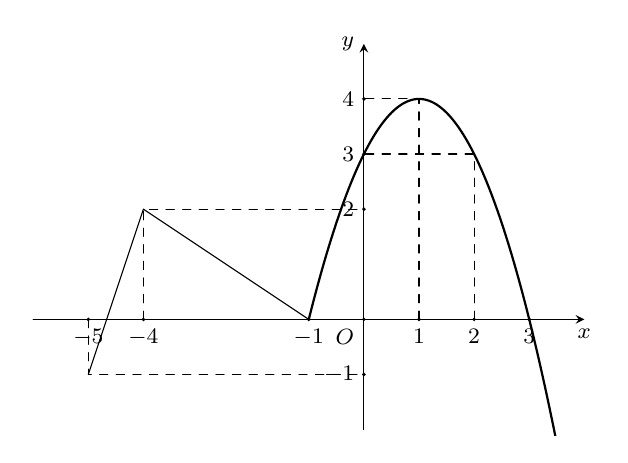
\begin{tikzpicture}[scale=0.7, font=\footnotesize, line join=round, line cap=round,>=stealth]
			%Gán số liệu.
			\def\xmin{-6};\def\ymin{-2};\def\xmax{4};\def\ymax{5};
			%Gán tọa độ.
			\coordinate (O) at (0,0);
			%Trục Oxy.
			\draw[->] (\xmin,0)--(\xmax,0) node[below]{$x$};
			\draw[->] (0,\ymin)--(0,\ymax) node[left]{$y$};
			\fill (O) node[below left]{$O$} circle(1pt);
			%Giới hạn đồ thị.
			\clip ({\xmin-0.1},{\ymin-0.1}) rectangle ({\xmax+0.1},{\ymax+0.1});
			\foreach \x in {-5,-4,-1,1,2,3}{
					\fill (\x,0) node[below]{$\x$} circle(1pt);
				}
			\foreach \y in {-1,2,3,4}{
					\fill (0,\y) node[left]{$\y$} circle(1pt);
				}
			\draw (-5,-1)--(-4,2)--(-1,0);
			\draw[thick,samples=100] plot[domain=-1:3.5](\x,{-(\x)^2+2*\x+3});
			\draw[dashed] (-5,0)|-(0,-1) (-4,0)|-(0,2) (1,0)|-(0,4) (2,0)|-(0,3);
		\end{tikzpicture}
	}
	\loigiai{
		Parabol $y=a x^2+b x+c$ qua các điểm $(2 ; 3)$, $(1 ; 4)$, $(0 ; 3)$, $(-1 ; 0)$, $(3 ; 0)$ nên xác định được $y=-x^2+2 x+3$, $\forall x \geq-1$ suy ra $f(x)=-\dfrac{x^3}{3}+x^2+3 x+C_1$.\\
		Mà $f(0)=0 \Rightarrow C_1=0$, $f(x)=-\dfrac{x^3}{3}+x^2+3 x$.\\
		Có $f(-1)=-\dfrac{5}{3}$, $ f(2)=\dfrac{22}{3}$.\quad $(1)$\\
		Đồ thị $f'(x)$ trên đoạn $[-4 ;-1]$ qua các điểm $(-4 ; 2)$, $(-1 ; 0)$.\\
		Nên $f'(x)=-\dfrac{2}{3}(x+1) \Rightarrow f(x)=-\dfrac{2}{3}\left(\dfrac{x^2}{2}+x\right)+C_2$.\\
		Mà $f(-1)=-\dfrac{5}{3} \Leftrightarrow C_2=-\dfrac{5}{3}+\dfrac{2}{3}\left(-\dfrac{1}{2}\right)=-2 \Rightarrow f(x)=-\dfrac{2}{3}\left(\dfrac{x^2}{2}+x\right)-2$, hay $f(-4)=-\dfrac{14}{3}$.\\
		Đồ thị $f'(x)$ trên đoạn $[-5 ;-4]$ qua các điểm $(-4 ; 2)$, $(-5 ;-1)$.\\
		Nên $f'(x)=3 x+14 \Rightarrow f(x)=\dfrac{3 x^2}{2}+14 x+C_3$.\\
		Mà $f(-4)=-\dfrac{14}{3} \Leftrightarrow \dfrac{3 \cdot(-4)^2}{2}+14 \cdot(-4)+C_3=-\dfrac{14}{3}$ suy ra $C_3=\dfrac{82}{3}$.\\
		Ta có $f(x)=\dfrac{3 x^2}{2}+14 x+\dfrac{82}{3} \Rightarrow f(-5)=-\dfrac{31}{6}$.\quad $(2)$\\
		Từ $(1)$ và $(2)$ ta được $2 f(-5)+3 f(2)=-\dfrac{31}{3}+22=\dfrac{35}{3}$.
	}
\end{ex}
\Closesolutionfile{ans}
% \indapan{10}{ans/ans-LC-2-C4B1CD3.1}